\documentclass{standalone}
\usepackage{tikz}
\usepackage{scalerel}

% \usetikzlibrary{positioning,chains,arrows}
\begin{document}
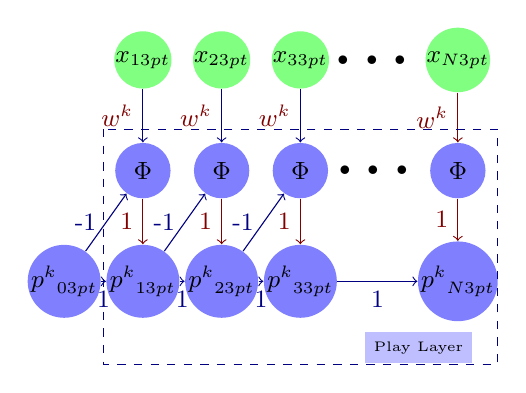
\begin{tikzpicture}[font=\small]
    % \draw (0.5,0.7) node [] {One Play};
    \tikzstyle{neuron}=[circle,fill=black!25,minimum size=20pt,inner sep=0pt];
    \tikzstyle{input neuron}=[neuron, fill=green!50];
    \tikzstyle{hidden neuron}=[neuron, fill=blue!50];
    \tikzstyle{activation neuron}=[neuron, fill=blue!50, rectangle, rounded corners=3pt, minimum size=13pt];
    \tikzstyle{play output neuron}=[neuron, fill=red!50, rectangle, rounded corners=3pt, minimum size=13pt];
    %% draw neurons
    \foreach \x in {1,2,3} {
        \node[input neuron] (x_\x) at (\x, 0) {$x_{\scaleto{\x}{3pt}}$};
        \node[hidden neuron] (phi_\x) at (\x,-40pt) {${\Phi}$};
    } 
    \foreach \x in {0,1,2,3}
        \node[hidden neuron] (p_\x) at (\x, -80pt) {${p^k}_{\scaleto{\x}{3pt}}$};

    \node[input neuron] (x_n) at (5,0) {$x_{\scaleto{N}{3pt}}$};
    \node[hidden neuron] (phi_n) at (5,-40pt) {$\Phi$};
    \node[hidden neuron] (p_n) at (5,-80pt) {${p^k}_{\scaleto{N}{3pt}}$};

    %% draw connections between nodes
    \foreach \x in {1,2,3} {
        \draw [->,color=blue!50!black] (x_\x) to node [left,color=red!50!black] {$w^k$} (phi_\x);
        \draw [->,color=red!50!black] (phi_\x) to node [left,color=red!50!black] {1} (p_\x);
    }
    \foreach \x / \y in {0/1,1/2,2/3} {
        \draw [->,color=blue!50!black] (p_\x) to node [left, color=blue!50!black] {-1} (phi_\y);
        \draw [->,color=blue!50!black] (p_\x) to node [below,color=blue!50!black] {1} (p_\y);
    }
    
    \draw [->,color=red!50!black] (x_n) to node [left,color=red!50!black] {$w^k$} (phi_n);
    \draw [->,color=red!50!black] (phi_n) to node [left,color=red!50!black] {1} (p_n);
    \draw [->,color=blue!50!black] (p_3) to node [below,color=blue!50!black] {1} (p_n);

    \path (x_3) -- (x_n) node[midway,scale=2,font=\bfseries] {\dots};
    \path (phi_3) -- (phi_n) node[midway,scale=2,font=\bfseries] {\dots};
    
    %% draw rectangle to include inputs/intermediate outputs
    \draw[dashed,thin,blue!50!black] (0.5,-25pt) rectangle (5.5, -110pt);
    \draw (4.5, -104pt) node [fill=blue!25!white] {\tiny Play Layer};

    % \draw[dashed,thin,green!50!black] (0.5,-12pt) rectangle (5.5, 12pt);
    % \node[] at (7, 0) {$X=[x_1,x_2,...,x_n]$};
    % \draw[dashed,thin,blue!50!black] (0.6,-68pt) rectangle (5.4, -92pt);
    % \node[] (op_output) at (2.8, -92pt) {};
    % \node[] at (7, -80pt) {$P=[p_1,p_2,...,p_n]$};
    

    % %% activation layer or non-linear layer
    % \begin{scope}[xshift=-13, yshift=-30]
    %     %% draw rectangle for non-linear layers
    %     \draw[dashed,thin,blue!50!black] (0,-105pt) rectangle (7, -136pt);
    %     \draw (6.05, -130pt) node [fill=blue!25!white] {\tiny Nonlinear Layer};
    %     %% draw rectangle for linear layers
    %     \draw[dashed,thin,red!50!black] (1.3,-142pt) rectangle (5.7,-171pt);
    %     \draw (4.9, -165pt) node [fill=red!25!white] {\tiny Linear Layer};

    %     % draw op output
    %     \foreach \s / \idx in {1/1,3/2} {
    %         \node[activation neuron] (activation_\idx) at (\s,-115pt) {\tiny $\tanh(\theta_{\scaleto{\idx}{2pt}}P+\theta_{\scaleto{\idx,0}{3pt}})$};
    %     }
    %     % draw non-linear node tanh(s)
    %     \node[activation neuron] (activation_s) at (6,-115pt) {\tiny $\tanh(\theta_{\scaleto{s}{2pt}}P+\theta_{\scaleto{s,0}{3pt}})$};
    %     % draw dots between two non-linear nodes
    %     \path (activation_2) -- (activation_s) node[midway,scale=2,font=\bfseries] {\dots};

    %     % draw play output
    %     \node[play output neuron] (play_output) at (3.5, -150pt) {\tiny $G^k=\sum_{s=1}^{S} \hat{\theta}_{\scaleto{s}{2pt}} \tanh(\theta_{\scaleto{s}{2pt}}P+\theta_{\scaleto{s,0}{3pt}}) + \hat{\theta}_{\scaleto{0}{2pt}}$};
        
    %     % draw connection between nonlinear layer and output layer, nonlinear layer and op_output layer
    %     \foreach \idx in {1,2} {
    %         \draw [->,color=blue!50!black] (op_output) to node [left,color=blue!50!black] {\tiny ${\theta}_{\scaleto{\idx}{2pt}}$} (activation_\idx);
    %         \draw [->,color=blue!50!black] (activation_\idx) to node [left,color=blue!50!black] {\tiny $\hat{\theta}_{\scaleto{\idx}{2pt}}$} (play_output);
    %     }
    %     \draw [->,color=blue!50!black] (op_output) to node [left,color=blue!50!black] {\tiny ${\theta}_{\scaleto{s}{2pt}}$} (activation_s); 
    %     \draw [->,color=blue!50!black] (activation_s) to node [left,color=blue!50!black] {\tiny $\hat{\theta}_{\scaleto{s}{2pt}}$} (play_output); 
    %     % draw connections \theta and \hat{\theta}
    % \end{scope}
\end{tikzpicture}
\end{document}
